\documentclass[12pt]{article}

%\usepackage{times}
%nips02e

\usepackage{spconf}
\usepackage{epsfig}
%\usepackage{psfig}
\usepackage{amsmath}
\usepackage[sort]{cite}
\usepackage{supertabular}
%\usepackage{dcolumn}
\usepackage{multirow}
\usepackage{rotating}
\usepackage{subfigure}
\usepackage{url}
\usepackage{bigstrut}
\usepackage{hhline}
%\usepackage{setspace}
%\usepackage{slashbox}
\usepackage[T1]{fontenc} % for bold small caps

\tolerance=1000
\hyphenpenalty=2000

%\textwidth 6.5in
%\textheight 9.0in
%\headheight 0.0in
%\headsep 0.0in
%\oddsidemargin 0.0in
%\evensidemargin 0.5in
\renewcommand{\topmargin}{-.25in} % AAA
\newcommand{\commented}[1]{}

%\global\boilerplate={}
%\global\copyrightetc{}

\newenvironment{packed_enum}{
\begin{enumerate}
  \setlength{\itemsep}{1pt}
  \setlength{\parskip}{0pt}
  \setlength{\parsep}{0pt}
}{\end{enumerate}}

\title{  AquaTux }
\name{David Biancolin, Adam Suban-Loewen, Victor Zhang, Ritchie Zhao}
\address{University of Toronto Mechatronics Design Association\\
email: mech.design@utoronto.ca }


\usepackage{comment}
% Un-comment one of the following two lines to turn pdf links on/off
%\includecomment{pdfrefs}
\excludecomment{pdfrefs}

\begin{pdfrefs}
\usepackage[ps2pdf]{hyperref}
% (See the hyperref package documentation for a list of supported drivers.)
\hypersetup{
    pdftitle={ AquaTux },
    pdfauthor={David Biancolin, Adam Suban-Loewen Victor Zhang, Ritchie Zhao},
    pdfsubject={AUVSI 2013},
    pdfkeywords={Mechatronics Design Association, AUV, submarine}
}
\end{pdfrefs}



%for subfigure
\renewcommand{\subfigcapskip}{0mm}
\renewcommand{\subfigtopskip}{0mm}
\renewcommand{\subfigbottomskip}{2mm}

\renewcommand{\topfraction}{0.999}     % max fraction of floats at top
\renewcommand{\bottomfraction}{0.99}        % max fraction of floats at bottom
\renewcommand{\floatpagefraction}{0.99}

\usepackage{amssymb}
\usepackage{fancyhdr}

\lhead{}
\chead{}
\rhead{}
\lfoot{}
\cfoot{Mechatronics Design Association -- University of Toronto}
\rfoot{\thepage}
\renewcommand{\headsep}{10pt}   %AAAA
\renewcommand{\headrulewidth}{2pt}
\renewcommand{\footrulewidth}{2pt}

\pagestyle{fancy}
\hyphenation{program-mable}
\hyphenation{pipe-lined}
\hyphenation{Chem-que}

\makeatletter
\renewcommand\maketitle{%
 \begin{minipage}[h]{.3\textwidth} 
   \centering 
   
\includegraphics[width=2in]{fig/logo2} 
 \end{minipage}% 
 \begin{minipage}[h]{.7\textwidth} 
   \centering 
\vspace{.3in}
\Huge{AquaTux} \\
\vspace{.1in}
\large{ David~Biancolin, Adam~Suban-Loewen, Victor~Zhang, Ritchie~Zhao }\\
\normalsize{ University of Toronto Mechatronics Design Association\\
 email: mech.design@utoronto.ca }

 \end{minipage} 
\vspace{.3in}
\par}
\let\after@maketitle\@empty
\makeatother
\begin{document}

%%%%%%%%%%%%%%%%%%%%%%%%%%%%%%%%%%%%%%%%%%%%%%%%%%%%%%%%%%%%%%%%%%%%%%%%%%%%%%%%

\twocolumn[\maketitle]



\thispagestyle{fancy} 

\begin{abstract}
%In the context of the AUVSI and ONR's Xth International Autonomous
%Underwater Vehicle Competition, the team at the University of Toronto
%built an underwater vehicle.

AquaTux is the fourth entry of the University of Toronto Mechatronics
Design Association into the annual Autonomous Underwater Vehicle
Competition.  The vehicle is designed to autonomously complete
the set of tasks described in the mission\footnotemark[1]. It is
equipped with a passive sonar system, an IMU, a depth sensor and
two cameras that allow it to navigate in its environment. This
year's frame was reused from previous years.
We are proud to present a new power system, more reliable electronics,
new embedded communication protocol using an FPGA, and new software.

\end{abstract}


\vspace{-.1in}
\section{Introduction} 

The construction of the vehicle that our team will present at the
2013 Autonomous Underwater Vehicle (AUV) competition encompasses several new achievements. We explain the
context of our realization by first describing the main
objectives of the competition and how our team is organized.


\subsection{Overview of the Mission}

The objective of the competition is to build an autonomous underwater
vehicle to perform various tasks involving image recognition, and
passive sonar to
interact with its environment. For the vision-guided tasks, the vehicle must 
pass through a validation gate, hit buoys, follow pipes,
pass through set of pipes, drop an object
in a box, launch a projectile through a hexagonal target, and manipulating a wheel.
The sonar tasks consists of
grabbing an object on top of an acoustic pinger and surfacing above it.
The details of the required tasks for the vehicle are described in the
 mission specification on the AUVSI website\footnote[1]{http://www.auvsifoundation.org/foundation/competitions/robosub/}.
Through the design and testing phases, emphasis was placed on
performing a subset of these tasks well rather than attempting all tasks.

\subsection{The Team}
The team consists of twenty members that are divided into three subsystems: mechanical, electronics, and software. In order to maintain a high degree of integration throughout the project, members are encouraged to work in projects that span multiple subsystems. Our hardware is obtained through sponsorship and funding from our university (see Section~\ref{ack}). 

Figure~\ref{organi} illustrates the major components of the AUV
and the reader should refer to it often as we describe the innovative
aspects of those components in the following sections.


\begin{figure*}
\begin{center}
 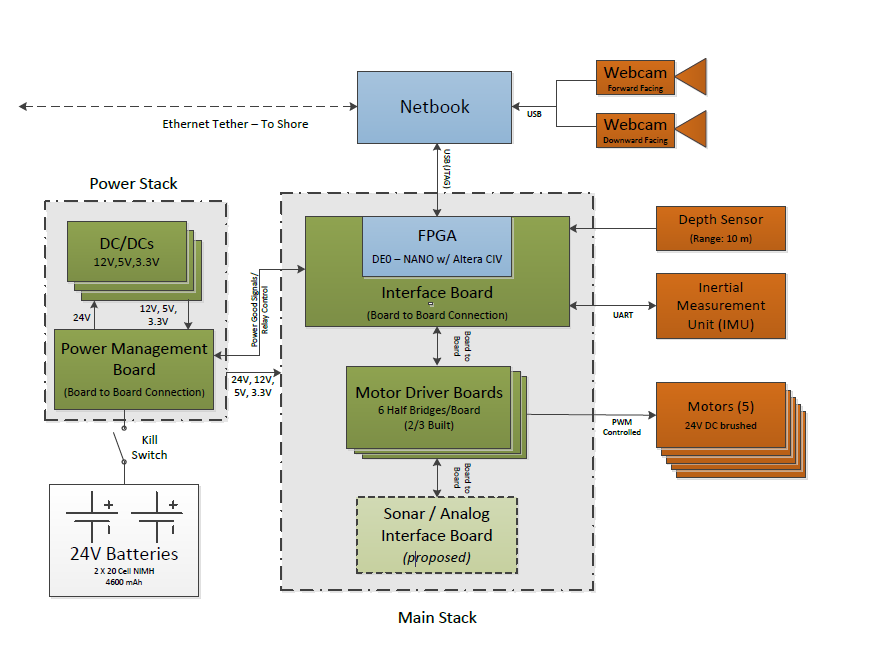
\includegraphics[height=3.7in]{fig/arch.png}
\caption{Organization of the AUV modules and their connectivity.}\label{organi}
\end{center}
\end{figure*}



\vspace{-.1in}
\section{Frame design and construction}
The 2009 frame design underwent a complete revision based on our
experience from previous years.  Our past frame designs included
custom ordered molded or rapid prototyped parts intended to improve
the hydrodynamics of the hull.  After analyzing the conditions that
the vehicle would be subjected to, it was determined that the effects
of fluid dynamics were negligible in terms of functionality.  For this
reason, a ``design for manufacturing'' development methodology was
adopted: in efforts to minimize cost and machining time, the frame has been
designed to take advantage of commercial off-the-shelf parts as
well as capitalize on simple manufacturing processes.

\subsection{Design Considerations}
\label{fobjectives}
The design objectives in the 2009 frame were significantly more
ambitious as our team included more members adept in manufacturing.
The final concept was conceived such that it could be fabricated
without the need for outsourcing.

Below is the list of the desirable attributes for the frame that we set out to
obtain based on the experience gained from past frame designs:
\begin{packed_enum}
\item Minimize time required to access batteries and electronics;
\item Maximize modularity for easier transport and progressive revisions;
\item Optimize mass for transport, functionality and points;
\item Provide a secure removable internal rack for electronics to facilitate bench testing;
\item Obtain a a waterproof seal with a simple low tolerance assembly;
\item Create solid harness points and handles;
\item Facilitate movement through water and maximize battery life with
  a neutrally buoyant design;
\item Compensate for changes in mass distribution and motion
  calibration with adjustable thruster positions;
\item Design an attractive and professional looking vehicle.
\end{packed_enum}

\subsection{Frame Overview}
The AquaTux frame design can be divided into three
subsections: external frame, hull, and internal rack.  The goals based
on past experience described above suggested the need to
minimize the number of sealing surfaces and reduce the number of
waterproof connectors.  To achieve these objectives, a single enclosure
was created (the hull) to encapsulate everything except for the
markers to be dropped, the thrusters and the hydrophones.  These external components would be
connected to an exoskeleton type frame which allows for flexible
mounting arrangements.  Finally an internal rack was designed to hold
 all the electrical components including cameras and embedded computer.

\subsubsection{External Frame}
The external frame was designed with transportation and fabrication as
the primary constraints. This exoskeleton is made entirely of
commercial off-the-shelf
parts, $\frac{1}{2}$ inch PVC plumbing pipe and connectors.  The thruster positions
are fully adjustable since they are attached to individual pipes fixed
in place by standard gear clamps (Figure~\ref{adj}). The adjustability of the frame also
facilitates transportation as the entire structure can be collapsed to
fit a smaller envelope. 

\begin{figure}
\begin{center}
 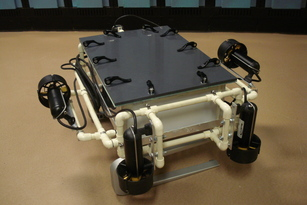
\includegraphics[width=3in]{fig/dsc06455} 
% 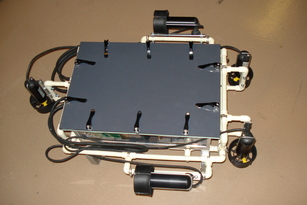
\includegraphics[width=3in]{fig/dsc06453} 
\vspace{.05in}
\hrule
\caption{Adjustable PVC tube exoskeleton frame.}\label{adj}
\end{center}
\end{figure}

In order to ensure a simple assembly method and utilize standard
connectors, the mechanism for picking up the briefcase was made of the
same material as the external frame.  It utilizes the fact that the
target is an open-walled structure and consists of a fork designed to
spear the case so that it can surface with the vehicle.

\subsubsection{Hull}
This year's hull design attempts to minimize the number of sealing
surfaces while maintaining usable space inside the vehicle.  In order
to seal the hull, a lid was made with a special simplified o-ring
groove (Figure~\ref{oring}). To avoid the need for precision milling or numerically
controlled machines, an oversized rectangular groove was cut.  The
corners were then drilled out and replaced with nylon dowels to
prevent the sharp corners from cutting into the o-ring.  This design
eliminated the need for specialized end mills or the need to mill
curved patterns in the lid. 

\begin{figure}
\begin{center}
 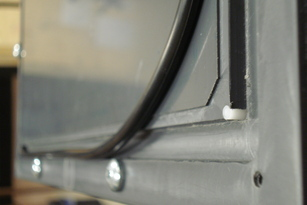
\includegraphics[width=3in]{fig/dsc06460.jpg} 
\vspace{.05in}
\hrule
\caption{O-ring displaced to show the grooves and nylon dowel.}\label{oring}
\end{center}
\end{figure}

Past experience suggested the need for a quicker method to access the
internal components of the hull.  Quick-release latches 
(Figure~\ref{quick}), were
used to replace nuts and bolts which take significantly more time to
release.  These latches use a cam mechanism to clamp the lid to
metallic bars and subsequently compress the o-ring, creating a water-tight seal.

\begin{figure}
\begin{center}
 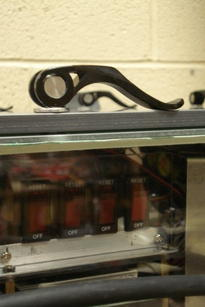
\includegraphics[width=1.34in]{fig/dsc06462} 
\vspace{.05in}
\hrule
\caption{Quick release cover mechanism.}\label{quick}
\end{center}
\end{figure}

An endplate was designed to provide a single replaceable surface to accept all the connectors between the interior and exterior of the vehicle.  This endplate is sealed with a groove similar to that of the lid and is attached with self sealing screws from APM Hexseal.  The waterproof connectors which pass through the endplate lead to two master-disconnects which allow for quick and easy installation of the internal rack (Figure~\ref{endplate}).
The waterproof connectors chosen are 8-pin Neoprene molded connectors
from Impulse Enterprise.  These connect the thrusters as well as the
wireless tether and provide maximal flexibility due to their pin count
as well as small profile.  
The pressure readings for the AUV are also gathered  through the
endplate. In order to sense depth, a MPX4115 pressure transducer is
coupled to a segment of PVC tubing connected to a compression nut on
the endplate.  The depth of the vehicle corresponds to the pressure of
the air trapped in the PVC tubing.
  The hull is fabricated from
$\frac{1}{8}$ inch thick polycarbonate sheets, with waterproof epoxy bonding
the joints together.  To strengthen the bonds, aluminum angle brackets
were added to the edges to increase the bonding area of the epoxy. The thin, clear polycarbonate walls of the hull allow subsystems such as the cameras, marker droppers (section~\ref{mdroppers}) and trigger for the torpedo to operate from within the vessel.

\begin{figure}
\begin{center}
\subfigure[Endplate showing waterproof connectors.]{ 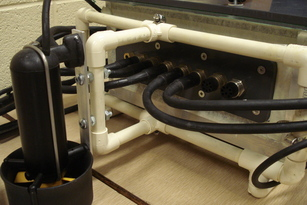
\includegraphics[width=3in]{fig/dsc06464} }
\subfigure[Master disconnects for the waterproof connectors on the
inside of the vehicle.]{ 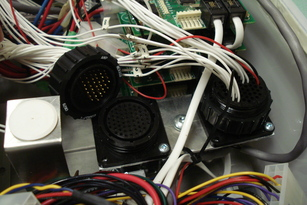
\includegraphics[width=3in]{fig/dsc06465} }
\vspace{.05in}
\hrule
\caption{Connection system to the outside of the vehicle.}\label{endplate}
\end{center}
\end{figure}

\subsubsection{Internal Rack}
In addition to remedying problems with our previous frames, we
endeavored to produce a frame that could be reconfigured and usable in
future years.  The concept for the internal rack (Figure~\ref{rack})
consists of base plates that accepts stacks of electronics.  These
plates can be removed as a single unit which facilitates wiring, and
bench testing.  Due to the buoyancy of the hull, stainless steel bars
were used to add weight to the vehicle (Figure~\ref{rack}).  These weights act as a method of balancing the
vessel and allow the electrical components to be reconfigured for
years to come.  The internal rack does not rest directly on the floor
of the hull.  In case of a leak, water would collect in the space
below the electrical components and be detected with leak sensors
prior to any damage.


\begin{figure}
\begin{center}
 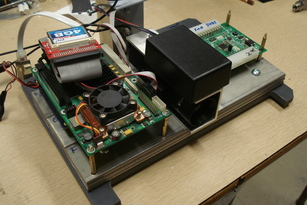
\includegraphics[width=3in]{fig/dsc06466} 
\vspace{.05in}
\hrule
\caption{Inside rack holding the electronics and the stainless steel weights.}\label{rack}
\end{center}
\end{figure}


\section{The Marker Dropper}
\label{mdroppers}

The thin walls of the hull facilitate the operation of a simple marker dropper system which
can be centered around the downward facing camera.  Two ferrous
markers are placed on the exterior of the vessel and held in place by
a magnetic attraction to two rare earth magnets located on the inside
of the hull.  The magnets are connected to individual stepper motors
which retract the magnets from the wall of the hull (Figure~\ref{md2}).  The increased
distance between the magnets and the markers causes a reduction in
magnetic field strength allowing the markers to drop freely from the
vehicle.

\begin{figure}
\begin{center}
 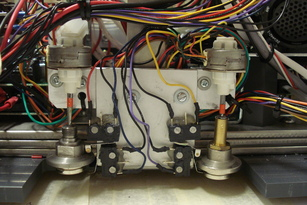
\includegraphics[width=3in]{fig/dsc06468} 
\vspace{.05in}
\hrule
\caption{Two marker-droppers: from top to bottom, a stepper motor
  retracts a magnet from the surface of the hull (bottom in the figure).}\label{md2}
\end{center}
\end{figure}

\section{The Torpedo Launcher}
\label{torpedo}
\vspace{-.1in}
One of the primary goals of this year's entry into the AUV Competition
was to minimize the number of connections that pass through the
endplate of the hull.  The resulting design for a torpedo launcher was
an external system that was activated by a magnetic switch.  This
concept allowed us to mimic the marker dropper design to activate the
torpedo.  The external system  contains only a few simple parts; a
power supply (9V battery), a solenoid valve, a magnetic switch, a
compressed gas cylinder and a projectile. As the magnet in the hull
is retracted from the hull, the magnetic switch is
triggered.  The switch  then triggers the solenoid valve allowing
compressed gas to fire the torpedo.

The controls for the above mentioned systems are described in the
following sections.

\vspace{-.1in}
%\section{Electrical aspects}

\section{Electronics and Communication}
Our electronics were designed to handle all low-level tasks that are
required to move AquaTux, acquire sensor data and trigger
electrical systems like the  marker droppers. The main goal
of the electronics is to allow the AUV to be driven with only
high-level heading and depth commands. The electronics are responsible for
executing the commands and controlling their results (e.g. depth or
heading) in a ``black box'' fashion. This level of separation, created by our command
communication protocol, provides the option of tethered communication directly to the Navigation board via RS232 or through the computer's ethernet port
that relays commands to the Navigation board.

\subsection{Navigation Board}
The Navigation Board provides signal conditioning and circuitry interfacing for all sensors, including the Motor Boards and Peripheral Control Boards. In addition, all communication either goes to or through the navigation board. This is also
the access point when the computer has to communicate with the lower level
electronics. It features an LPC2129 microcontroller (MCU) at its core, operating at
12Mhz and utilizes Control Area Network (CAN), two-wire serial I2C,
and RS232 protocols to communicate with the Motor Boards, Peripheral
Control Board / Batteries, and the Computer respectively. The
navigation board reads the heading from an HMR3300 Digital Compass
connected through a serial port.  An analog pressure sensor, MPX4115, provides a linear
voltage representation of the depth, and is also connected to the
navigation board feeding directly into a successive approximation A/D
in the LPC2129. This board is the key element in handling all low-level operations such as movement and data collection.

\subsection{Peripheral Control Board}


The circuit board operates as an extension to the navigation board by
performing the tasks of actuating the marker droppers and debouncing
the custom-made leak sensors. The Peripheral Control Board uses
SN754410 quadruple half H-Bridge drivers: two of which are used to
actuate the marker droppers and one to fire the torpedo. The
Peripheral Control Board uses an ATmega48p MCU to control the half
H-bridge drivers, and query the leak sensors and the feedback switches
from the marker dropper. The microcontroller communicates with the
navigation board through the I2C network of the AUV.

\subsection{Motor Board}

The motor drivers are used to control the Seabotix BTD150 Thrusters
used on AquaTux.  There are a total of five motor drivers, one for
each thruster used on the AUV (Figure~\ref{mstack}). The motor drivers are based around the NXP
LPC2129 MCU which has number of features ideally suited to our
application, including a 4 channel SAR ADC, a 6-channel dual edge
triggered PWM module, a CAN module and a simple serial boot-loader.
The thrusters are controlled via current control, and other safety
features such as current limiting, and acceleration control are
implemented.  By receiving commands through the CAN bus, these Motor
Boards will ensure that the thrusters are never harmed by excessive
current during operation.

\begin{figure}
\begin{center}
 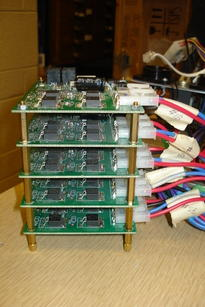
\includegraphics[width=1.5in]{fig/dsc06472} %1.34
\vspace{.05in}
\hrule
\caption{Stack of motor control boards on a CAN bus.}\label{mstack}
\end{center}
\end{figure}


The motor controller hardware is centered around a pair of Linear
Technology LT1160 half-bridge drivers which include high side charge
pumps, shoot through protection and undervoltage lockout. A number of
additional components were added to increase the bridge robustness
including TVS diodes, anti-parallel gate diodes and large on-board
bulk capacitors. Two types of sensors were integrated into the motor
board in order to sense motor function. Back EMF measurement
capability as well as motor current circuits were added. An active-RC
filter similar to that on the navigation board was used coupled with a
high side sense resistor and INA168 to measure the motor current.
Motor current measurement is critical as it must be kept below 4A to
prevent motor damage.

\section{Power Distribution}
AquaTux is powered by three 24V NiMH battery packs.  The three battery
packs each power a different section of the AUV.  Two packs directly
feed into the Motor Boards: one pack is used to power the three
vertical thrusters, and a second pack provides power for the two
horizontal thrusters.  The last battery pack provides power for the
rest of AquaTux after being conditioned by Switch Mode Power Supplies
(SMPS) to create two separate bus voltages. A 5V SMPS feeds the
Kontron SpeedMopsLcdPM PC104+ computer, while a 12V SMPS provides power to
all other modules of the AUV, which includes the navigation board,
cameras, and all other sensors. If other voltages are required for the
electronics, linear regulators are used to produce them.  In case of
emergency, relays toggled by magnetic switches are used to disconnect
the batteries from the rest of the AUV. Circuit breakers are also put
inline with the battery to act as both the fuse, and the power
switches for the AUV. The power architecture was designed to keep
board to board wiring simple by minimizing the number of bus voltages.

\subsection{Power Source}
The NiMH battery packs were custom designed by our team: each pack is
composed of 20 SY136T Sanyo nickel metal hydride batteries.  All
batteries are connected in series to form a 24V nominal battery pack
with a capacity of 4100mAh.  Each pack has its own protection
circuitry that utilizes an Atmega48p AVR as its MCU.  A gas gauging IC, BQ2013,
from Texas Instruments is used to track the charge status of the
battery. %BQ2013
For safety, the pack has a disconnect FET on the high side of the
battery.  This FET will disconnect the pack when the pack is drained
or at a temperature greater than 80 degrees Celsius. All battery packs
are connected to the I2C bus on the navigation board, allowing for
remote monitoring of the batteries at all time.

\subsection{Battery Charger}
The battery charger was also designed by our team and has at its core
an Atmega168p MCU.  This MCU monitors the voltage and
temperature of the battery pack being charged, and will automatically
terminate charging based on the temperature rise of the NiMH cells.
The charger must also communicate with the pack via I2C in order to
read the battery pack ID, and to ensure that the disconnect FET is
enabled for charging.  Charge current is set by utilizing a sense
resistor, and an opamp to control the gate voltage of a MOSFET.  The
MOSFET operates in saturation in order for us to appropriately limit
the charge current of the batteries. Because the voltage range of the
NiMH cells extends from 1.4V to 1.6V, the voltage supply required to
charge a 20 cell pack must be greater than 32V: we chose a 36V supply for cost-effectiveness.

\vspace{-.1in}
\section{Embedded System}

The embedded system was designed to link the submarine's computer with all
electronic peripherals, with a high-level interface to access groups of peripherals.
The embedded system consists of a DE0-Nano FPGA, synthesizing custom circuitry to
communicate with each peripheral and a soft processor to communicate with the computer. The FPGA was chosen
for its quantity of general-purpose I/O pins, allowing it to manage all electronic peripherals,
and its compact size of 3x2 inches. The FPGA is the only programmable element in the submarine
besides the computer, reducing the amount of communication between programmable elements.

\subsection{FPGA Soft Processor}

The FPGA Soft Processor exposes high-level commands to the computer to access each group
of electronic peripherals.
The IMU and depth sensor provide attitude readings and are used by the PID controllers and the
computer interface. Power management continually monitors each
voltage rail, and will power off the submarine if any voltage is invalid.
The five motor drivers are controlled together by the soft processor's yaw, pitch, roll,
and depth PID controllers. The computer interface can set target
speed, yaw, and depth, which are inputs to the PID controllers. Speed is implemented as an offset
because the submarine does not have velocity measurement. The PID controllers are implemented on the
soft processor because they need immediate access to the motor drivers and attitude readings.
The high-level commands are
text-based, allowing manual control to test each peripheral individually.
Future plans for sonar processing will be implemented on the FPGA, using the soft processor and
built-in DSP elements.

\subsection{FPGA Hardware}

The FPGA also synthesizes custom hardware to communicate with peripherals through general-purpose pins.
This flexibility can support any protocol to communicate with peripherals, including SPI and UART.
Each peripheral protocol is a separate module, memory-mapped to the soft processor across Altera's
Avalon Bus. The DE0-Nano has 85 general-purpose pins for digital inputs and 8 ADC inputs.
The depth sensor is an analog peripheral, and all other peripherals communicate digitally.
The hardware and soft processor run at 50 MHz.

\vspace{-.1in}
\section{Software}

The submarine's software is aware of the competition objectives, and performs computer vision to
command the submarine to move through the embedded system.
The computer vision uses the OpenCV library to help identify objects based on shape and color.
The video input consists of two webcams, one facing forward and one facing down.
These cameras are rigidly attached to the AUV, and the AUV must move to change the viewpoint.
The software also includes a graphical simulator that we can use to test our computer vision algorithms.

\subsection{Software Organization}
\label{gui}


\begin{figure}
\begin{center}
 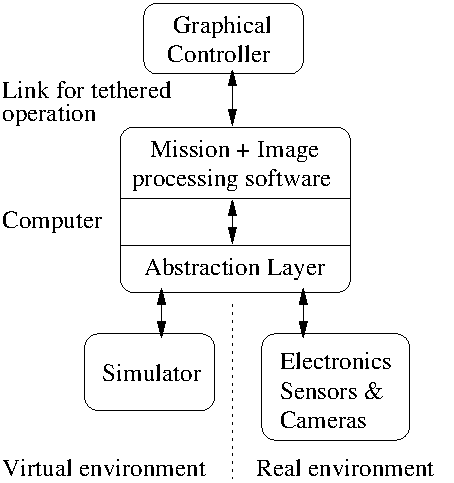
\includegraphics[width=2.2in]{fig/vision}
\caption{Software module organization.}\label{vision}
\end{center}
\end{figure}


\begin{figure}
\begin{center}
 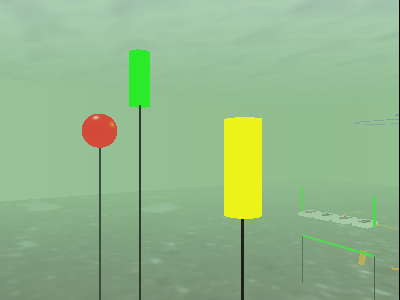
\includegraphics[width=2.7in]{fig/sim.png}
\caption{Example image from the simulator showing pipe segments and the buoys
         in turbid water.}\label{sim}
\end{center}
\end{figure}

The software is broken down into 3
components (Figure~\ref{vision}): (i) the mission software that performs the image
processing; (ii) the simulator that recreates synthetic underwater
images based on the vehicle position (example in
Figure~\ref{sim}) and (iii) the graphical interface that is used to
control the mission software. The simulator and the graphical
interface were solely created to test and debug the vision
algorithms when AquaTux is not functioning autonomously. All modules connect through TCP/IP in a
very flexible and extensible fashion. This allows us to seamlessly
replace the simulator by the real hardware sensors and electronics
when we take our system from the lab to the water environment. The
graphical interface allows us to access all the data structures in the
AUV and can act as a passive observer, constantly requesting the
state of the vehicle, or as a controller sending commands to the
vessel.



\vspace{-.1in}
\subsection{Image Processing Software}
The image processing software consists of color filters and edge and
line detection algorithms. The color filters allow us to select
specific information to only process relevant parts of the images. The
line processing algorithms use heuristics to form polygons and
recognize objects such as pipes or boxes, that have a well defined
appearance. Our algorithms are robust enough to recognize objects even
if their view changes due to perspective or the presence of debris in
the water.  The mission software consists of a main loop that acquires
images, processes them and send commands to the other subsystems on
one of the two serial ports of the embedded computer (see
Section~\ref{gui}). The mission is broken down into modular tasks that
can me chained or tested individually. Tasks proceed by first
identifying a target for the vehicle to begin pursuit. If the object
in question is not found, the vehicle rotates on its vertical axis
(yaw) to make the cameras pan to the right and to the left. If nothing
is found, then the vehicle proceeds forward in its initial direction.
Once a target is acquired, the vertical position and lateral positions
of the vessel are controlled to match the desired coordinates.  The
vehicle uses a combination of heading relative to its current
orientation and absolute headings (relative to the magnetic north
pole) to navigate inside the environment. This alleviates the need to
get real-time measurements of the heading as the vehicle is
navigating. A limitation of our vision hardware that we had to address
is to determine when a task is completed if the view of the target is
obscured or occluded due to the AUV's proximity (e.g. it is passing
under the gate). In such situations, for the moment being, we use
timers to ensure that the vehicle reaches its target location.

\vspace{-.12in}
\section{Conclusions} 
\vspace{-.03in}

This year's team took on the challenge of building a completely new
autonomous underwater vehicle: AquaTux. This AUV is composed of an embedded
computer that is linked to an interconnection of microcontrollers. More emphasis was directed towards the frame to
ensure that the electronics remain dry. While a lot of the design
decisions are influence by our past experience, we also learned many
techniques and principles over the last year. Circuit board
fabrication, plastic machining and software engineering are some of
the skills that many of our members were able to acquire. More
rational design techniques and project management skills are also
derived from the our previous competitions and they had a significant
effect on maximizing the productivity of all the man-hours contributed
to the project.


\vspace{-.12in}
\section{Acknowledgments}
\label{ack}
\vspace{-.03in}

We would like to thank the staff of the University of Toronto for
supporting our project.

We would also like to thank all our sponsors who have helped make this
project possible: The University of Toronto Engineering Alumni
Association, The Edward S. Rogers Department of Electrical and
Computer Engineering, The Division of Engineering Science, the
University of Toronto Engineering Society, and Altera.

%\vspace{-.08in}
\small
%\bibliographystyle{IEEEtran}
%\bibliography{IEEEabrv,paper}


\end{document}
